\documentclass[journal]{IEEEtran}
\usepackage[T1]{fontenc}
\usepackage{amsmath,amssymb,graphicx,booktabs,array,multirow,cite}
\usepackage{balance}
\usepackage[hidelinks]{hyperref}
\hypersetup{pdftitle={Hierarchical RF Tokenization for Parameter-Efficient Cross-Receiver LoRa Identification},pdfauthor={Anonymous review draft}}
\graphicspath{{figures/}}
\newcommand{\method}{HStem}
\newcommand{\pp}{\,\mathrm{pp}}
\newcommand{\R}{\mathbb{R}}
\hyphenation{finger-print finger-printing token-ization}
\begin{document}
\title{Hierarchical RF Tokenization for Parameter-Efficient\newline Cross-Receiver LoRa Identification}
\author{Anonymous review draft}
\maketitle

\begin{abstract}
Radio-frequency fingerprint identification must distinguish transmitters despite receiver-dependent distortion and limited labeled source data. This paper studies how RF tokens should be formed under a fixed, strictly in-band LoRa representation. A four-stage hierarchical convolutional tokenizer, followed by two ordinary multi-head attention blocks, replaces a large single-stride patch projection while preserving a 32-token, 64-channel interface. On an existing two-fold, three-seed development protocol, the resulting model achieves 97.335\% receiver-equal accuracy with 133,690 parameters, compared with 95.222\% and 571,434 parameters for the full patch model. Against a parameter-matched grouped patch control, the gain is 2.687 percentage points. Controlled ablations show that full-rank kernel reparameterization and additional local support each affect performance; restoring affine parameters alone does not recover the full hierarchical model. A trained round-trip interpolation operator can be materialized as an ordinary convolution with bitwise-identical logits on 12,000 source-validation evaluations. We also report computational costs, precision-dependent batch-normalization folding, and substantial sensitivity to small digital shifts. The evidence supports parameter-efficient token construction for the present aligned LoRa protocol. It does not establish receiver-hardware invariance, synchronization robustness, or new independent receiver confirmation.
\end{abstract}
\begin{IEEEkeywords}
RF fingerprint identification, LoRa, cross-receiver recognition, tokenization, parameter efficiency.
\end{IEEEkeywords}

\section{Introduction}
\IEEEPARstart{R}{adio}-frequency fingerprint identification (RFFI) classifies transmitting devices using differences present in received waveforms. Receiver circuitry and propagation conditions also influence those waveforms. Consequently, a representation that separates transmitters on one receiver can fail on another. Multi-receiver LoRa studies have demonstrated the importance of this problem and investigated receiver-adversarial learning and collaborative inference~\cite{shen2024}.

This paper considers a more specific design question: with a fixed signal representation and a small source-data budget, how should a sequence model form RF tokens? A large patch convolution can compress a long input to a short token sequence, but allocates many parameters to a single projection. Hierarchical convolutions offer a different allocation of local processing, downsampling, normalization, and nonlinearities. Their use is well established in other sequence and vision applications~\cite{cvt2021}. Their effectiveness for a particular RF representation must nevertheless be demonstrated with controls that distinguish parameter count from structural changes.

We study this question using an inherited strictly in-band, five-channel LoRa front-end~\cite{prioroob}. The front-end is held fixed. The proposed \method{} tokenizer progressively maps 8,192 feature positions to 32 tokens of dimension 64, followed by two ordinary multi-head attention (MHA) blocks. We use a large patch baseline and a grouped, parameter-matched patch control. Subsequent interventions examine expanded local support, invertible kernel reparameterization, and intermediate batch normalization (BN).

The evidence is useful but has a defined scope. The consolidated experiments reuse an existing development corpus and a previously examined historical receiver set. The comparison is source-only during model fitting, but the overall research process has used the development results repeatedly. It is therefore a controlled development study rather than a fresh blind evaluation. Furthermore, fewer parameters do not imply lower computation: \method{} increases counted multiply-accumulate operations (MACs) relative to the matched patch control. Small digital shifts cause substantial degradation in both models. These results are reported as part of the method's applicability, rather than hidden behind mean accuracy.

The contributions are as follows.
\begin{enumerate}
\item We specify a parameter-efficient hierarchical RF tokenizer for a fixed, strictly in-band LoRa pipeline, and compare it with full and parameter-matched patch constructions under the same training recipe and token interface.
\item We provide controlled evidence that kernel parameterization and local-support-related design both influence cross-receiver performance. The interventions narrow possible explanations without claiming a unique hardware or anti-aliasing mechanism.
\item We separate training parameterization from deployment structure through convolution materialization and precision-qualified BN folding, and document receiver-level performance, computational costs, and alignment sensitivity.
\end{enumerate}
The second and third contributions support the central tokenizer design; they are not presented as two additional original learning algorithms.

\section{Related Work and Inherited Components}
\subsection{Cross-Receiver RF Identification}
Shen \emph{et al.} study receiver-agnostic LoRa identification, collaborative receivers, and adaptation~\cite{shen2024}. Recent approaches also address nuisance information through information-bottleneck regularization~\cite{ibrff2026} and channel/receiver robustness through learned signal representations and contrastive objectives~\cite{ma2025}. A separate line combines channel processing, metric-based confidence, and model compression~\cite{light2026}. These approaches motivate strong comparisons, but their published percentages cannot be transferred to our source budget or receiver partition. We retain historical same-corpus results separately from the paired tokenizer experiments, with their implementation and selection differences disclosed in the supplement.

Our method does not introduce receiver-adversarial optimization, information-bottleneck regularization, test-time adaptation, or an additional loss. The experimental question concerns token construction within a shared signal pipeline. A separate Wi-Fi investigation is outside the claims of this paper.

\subsection{Convolutional Tokens, Normalization, and Stability}
Convolutional token embeddings and hierarchical feature processing predate this study~\cite{cvt2021}. MHA is likewise a standard component~\cite{attention2017}, as is BN~\cite{bn2015}. We do not claim novelty for these components individually. The contribution is the specified LoRa configuration and the evidence that its performance persists against a close parameter-budget control.

Work on shift stability shows why downsampling and invariance require explicit scrutiny~\cite{zhang2019}. It does not imply that a hierarchical RF network is shift stable. Our shift experiments demonstrate the opposite for the present representation and aligned-window protocol.

\subsection{Relationship to the Related OOB Study}
The related OOB-dependence manuscript~\cite{prioroob} investigates frozen-model sensitivity to out-of-band pathways. We inherit its strict in-band projection, five-channel representation, convolutional front-end, and 32-by-64 token interface. We also use the same public LoRa corpus. These are shared foundations, not new contributions of this paper. Our question is token formation under a strictly in-band pathway, with no OOB fusion. The supplement provides a component-level overlap statement. The six receivers called blind in the earlier work have already been used there and are not new blind receivers for this study.

\section{Signal Representation and Token Construction}
\subsection{Task and Fixed Front-End}
Let $x\in\mathbb{C}^{8192}$ denote a fixed received window and $y\in\{1,\ldots,10\}$ its transmitter label. Training uses labeled source receivers. Inference uses the same closed transmitter set on receivers excluded from that fitted model. No samples from an evaluation receiver are used to update model parameters, normalization statistics, checkpoints, or the learning-rate schedule of that model.

The inherited front-end normalizes packet RMS and applies the fixed projection
\begin{align}
 \widetilde{x}&=\mathcal{F}^{-1}\!\left[M\odot\mathcal{F}(x/\operatorname{RMS}(x))\right],\\
 M_k&=\mathbf{1}\{|f_k|\leq62.5\,\mathrm{kHz}\}.
\end{align}
The sampling rate is 1 MHz and the nominal LoRa bandwidth is 125 kHz. All downstream views are reconstructed from $\widetilde{x}$. The five channels contain I/Q, FFT magnitude, and amplitude/phase views, with the inherited normalizations unchanged. The FFT channel is a magnitude view, not explicit spectral phase. The phase view is the time-domain $\operatorname{atan2}$ phase. Dataset CFO and SNR metadata are not model inputs.

Two shared stride-one convolutions, with kernels 7 and 5 and 32 output channels, use BN and LeakyReLU. Their output is $h\in\R^{32\times8192}$. A channel index shared by temporal and spectral views is a feature coordinate; it should not be interpreted as a uniquely localized physical time interval. In particular, FFT and band projection are global operations.

\begin{figure*}[t]
\centering
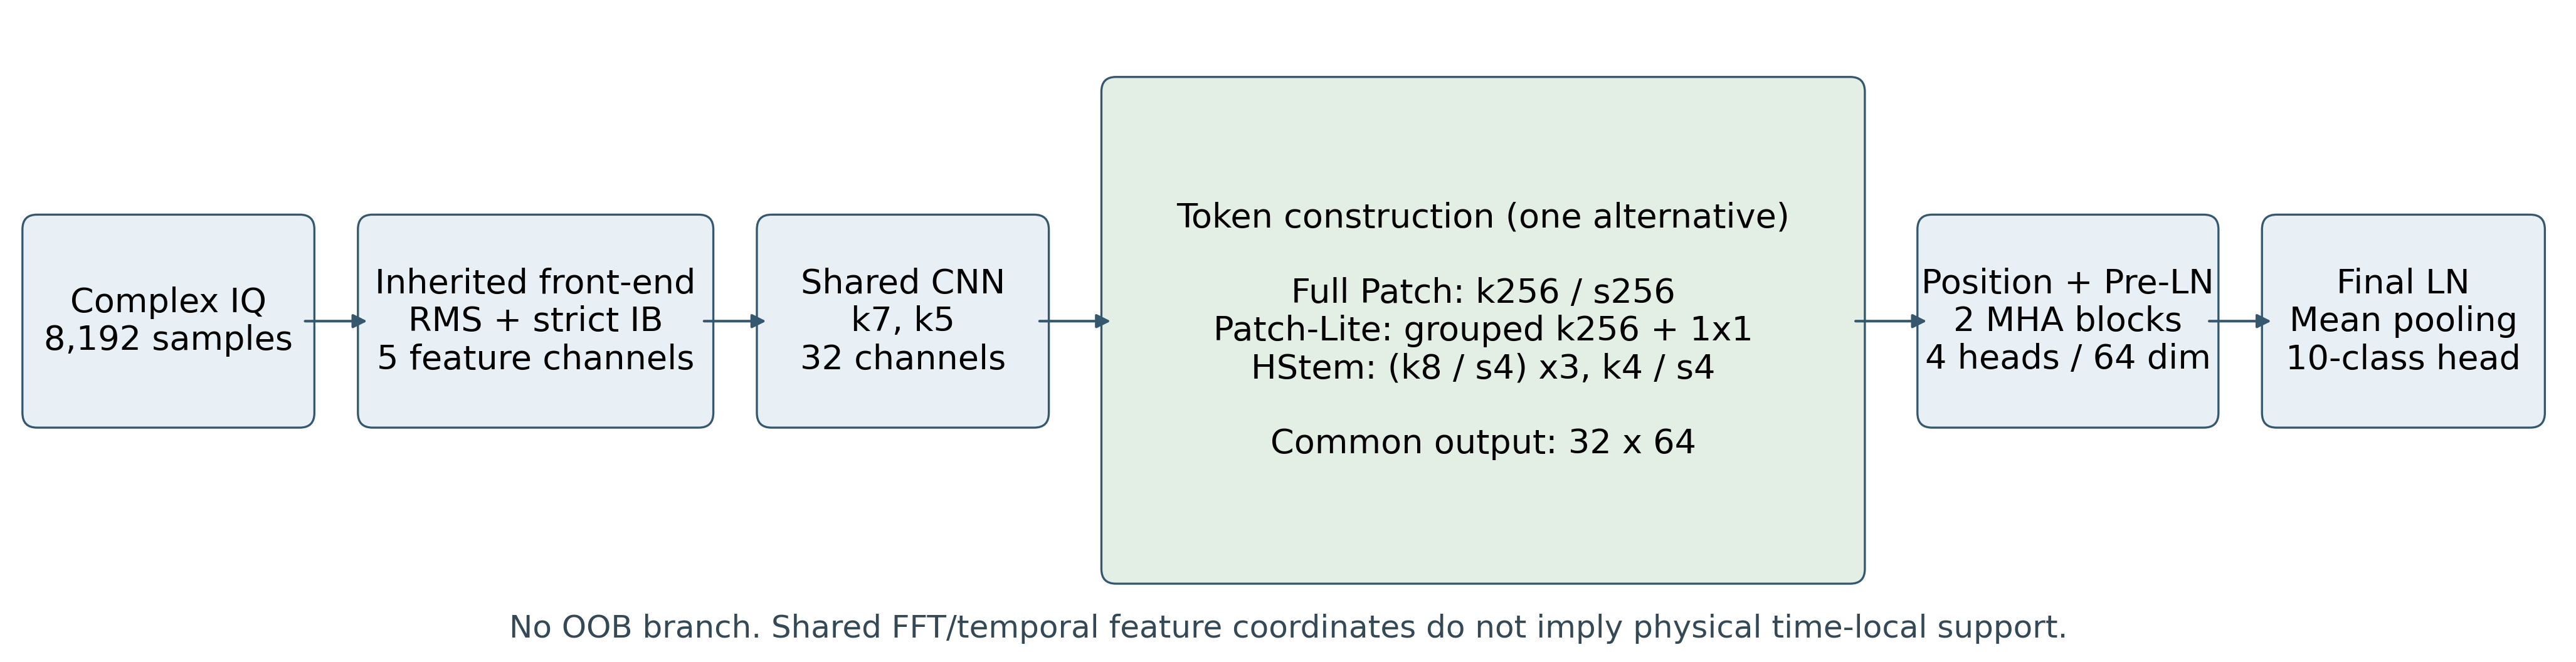
\includegraphics[width=.97\textwidth]{architecture.png}
\caption{Fixed signal pathway and alternative tokenizers. Only token construction changes in the main comparison. The hierarchical branch retains the 32-by-64 interface of the patch controls. Feature-coordinate support does not equal end-to-end physical RF support.}
\label{fig:architecture}
\end{figure*}

\subsection{Hierarchical Tokenizer}
\method{} applies four convolutional stages. The first three have kernel 8, stride 4, padding 2, and output widths 48, 64, and 64. Each is followed by BN and GELU. The final stage has kernel 4, stride 4, no padding, and output width 64. The lengths are
\begin{equation}
8192\rightarrow2048\rightarrow512\rightarrow128\rightarrow32.
\end{equation}
The output is transposed to 32 tokens in $\R^{64}$. The token stride is 256 and the first token center is 127.5 in zero-based feature coordinates. Including the shared local front-end, the CNN support is 350 positions. These geometric quantities describe the convolutional feature pathway only.

The same input projection, learned positional embedding, and pre-normalization are retained for all MHA comparisons. Each of two attention blocks uses four heads and a projected width of 64. A block computes softmax scaled dot-product attention, an output projection, a residual addition, and layer normalization. This is an ordinary attention block without a feed-forward expansion. Final layer normalization, mean token pooling, and a linear 10-class classifier complete the model.

\subsection{Full and Parameter-Matched Patch Controls}
The full patch control uses a single kernel-256, stride-256 convolution from 32 to 64 channels. It has the same token count and MHA head, but 571,434 total parameters. The parameter-matched Patch-Lite uses a grouped kernel-256 convolution from 32 to 80 channels with eight groups, followed by a 1-by-1 projection to 64 channels. Its 134,266 parameters are within 0.44\% of \method{}'s 133,690. The configuration was selected by a data-free parameter-count search with a 1\% tolerance, not by evaluation accuracy.

The matched control limits a simple capacity explanation. It does not isolate hierarchy alone: grouping, support, intermediate normalization, nonlinearities, and arithmetic cost remain different. Both patch controls have CNN support 266; token stride and center are unchanged.

\section{Controlled Mechanism Interventions}
\subsection{Expanded Support and Full-Rank Parameterization}
Overlap-Patch retains the learned grouped kernel $w$ of Patch-Lite. Fixed linear interpolation expands each kernel from 256 to 340 positions, scales it by $\sqrt{256/340}$, and uses stride 256 with padding 42. Learned parameter count, token centers, and token count remain unchanged, while CNN support increases to 350. Expansion also changes the operator's frequency response, so this is not a pure intervention on support.

The Smooth-RoundTrip control uses the same expansion followed by fixed interpolation back to 256 positions. It has the original support 266 and the same learned parameters as Patch-Lite. In vector notation its effective kernel is
\begin{equation}
v=T w,\qquad \operatorname{rank}(T)=256.
\label{eq:parameterization}
\end{equation}
Thus it preserves the expressible 256-position kernel space while changing initialization and optimization coordinates. The singular values of $T$ range from approximately 0.3892 to 0.9178. A center-crop proposal was rejected by a data-free rank audit before its scientific training; the trained control is the full-rank round-trip version.

For ordinary gradient descent, the effective-kernel update would contain $TT^{\mathsf T}$ as a preconditioner. Our models use AdamW~\cite{adamw2019}; the ordinary-gradient-descent identity is not an exact AdamW update. Kernel spectra and local gradient calculations are supporting diagnostics, not a complete causal explanation of the optimizer's behavior.

\subsection{Normalization Controls}
NoMidBN removes the three BN layers inside the hierarchical tokenizer while preserving the two shared front-end BN layers. AffineOnly replaces those same three BN layers with learned per-channel scale and offset, initialized to one and zero. AffineOnly restores 352 learned parameters without restoring batch or running-statistic normalization. These comparisons test whether parameter restoration alone is sufficient; they do not separately identify batch statistics, running statistics, and optimization dynamics.

\subsection{Deployment Materialization}
Equation~\eqref{eq:parameterization} permits a trained Smooth-RoundTrip kernel to be stored directly as an ordinary convolutional kernel. No interpolation is then required during inference. Separately, a frozen BN layer after a convolution can be folded by
\begin{align}
W'_c&=\frac{\gamma_c W_c}{\sqrt{\sigma_c^2+\epsilon}},\\
b'_c&=\beta_c+\frac{\gamma_c(b_c-\mu_c)}{\sqrt{\sigma_c^2+\epsilon}}.
\end{align}
These algebraic operations preserve the trained function in exact arithmetic. Backend precision must still be tested. Folding a trained BN is not equivalent to training NoMidBN from scratch.

\section{Experimental Protocol}
\subsection{Data, Receivers, and Historical Exposure}
The source corpus contains 10 LoRa transmitters and 20 SDR receivers~\cite{shen2024}. We use the frozen P-H5x160 protocol. Two complementary source/development folds each use five source receivers and five development receivers. From each source receiver and transmitter, 160 selected packets train the model and 40 select its checkpoint, giving 8,000 training and 2,000 validation packets per fold. Development evaluation uses 200 packets per transmitter and receiver. Four additional receivers form the historical-confirmation group. Receiver lists and exact selection rules appear in the supplement.

The development receivers are excluded from fitting their evaluated model, but have been used for method development across stages. The four historical-confirmation receivers also have prior exposure. The six receivers reserved from the current protocol were used in the earlier OOB study and remain unopened here. Neither the historical-confirmation set nor those six receivers supplies a newly independent blind test.

\subsection{Training and Model Selection}
Each configuration uses two folds and three paired seed labels, 201, 202, and 203. Data order and noise streams are paired within a fold and seed. Models train for 200 epochs with batch size 64, AdamW, peak learning rate $10^{-3}$, weight decay $5\times10^{-4}$, five-epoch linear warm-up, and cosine decay. Training adds AWGN with a per-packet nominal ratio sampled uniformly from 0 to 50 dB. This is added noise relative to observed packet power, not a measured physical SNR. The checkpoint minimizes receiver-equal cross-entropy on source validation only; all 200 epochs run.

The current paper consolidates already completed stages. For each mechanism stage, new checkpoints were selected and sealed before its development and historical-confirmation evaluation. This chronology protects within-stage fitting decisions but does not make the cumulative research process an independent confirmation. No new training is performed for manuscript preparation.

\subsection{Metrics and Conditional Uncertainty}
The main metric averages packet accuracy equally across evaluation receivers,
\begin{equation}
 A_{\mathrm{RX}}=\frac{1}{|\mathcal R|}\sum_{r\in\mathcal R}
 \frac{1}{N_r}\sum_{i\in r}\mathbf{1}\{\hat y_i=y_i\}.
\end{equation}
We report macro-F1, cross-entropy, seed variation, worst-receiver accuracy, paired differences, and TX-by-RX error changes. Receiver-cluster bootstrap intervals average training repeats within each receiver. Development intervals use 10 receivers; historical-confirmation intervals use four. Six positive fitted pairs means two folds times three seeds, not six independent receivers. Intervals condition on the fitted seeds and development design, with no multiplicity correction.

Four mechanism contrasts were fixed before their corresponding new results: Overlap minus Smooth-RoundTrip, Smooth-RoundTrip minus Patch-Lite, \method{} minus AffineOnly, and AffineOnly minus NoMidBN. A practical signal required at least 0.5 pp mean improvement, positive differences in both folds, at least five of six positive fitted pairs, an RX-cluster interval above zero, and a worst-RX difference no lower than -2 pp. The complete rules and non-passing results are retained.

\section{Results}
\subsection{Parameter-Efficient Cross-Receiver Identification}
\begin{table}[t]
\centering\caption{Consolidated MHA results. Dev: development RX; Hist.: historical confirmation with prior exposure. SD is across three seed means, each averaged over folds.}
\label{tab:main}
\setlength{\tabcolsep}{3pt}\footnotesize
\begin{tabular}{lrrrr}
\toprule Model & Params & Dev (\%) & SD & Hist. (\%)\\\midrule
Full Patch & 571,434 & 95.222 & 0.415 & 93.685\\
Patch-Lite & 134,266 & 94.648 & 0.137 & 93.367\\
Smooth-RoundTrip & 134,266 & 95.527 & 0.418 & 94.050\\
Overlap-Patch & 134,266 & 96.345 & 0.396 & 94.942\\
NoMidBN & 133,338 & 96.145 & 0.265 & 95.458\\
AffineOnly & 133,690 & 96.417 & 0.752 & 95.352\\
HStem & 133,690 & 97.335 & 0.308 & 96.508\\
\bottomrule\end{tabular}
\end{table}

Table~\ref{tab:main} shows that \method{} reaches 97.335\% development accuracy with 133,690 parameters. The full Patch model reaches 95.222\% with 571,434 parameters: a 76.60\% parameter reduction and a descriptive 2.113 pp accuracy increase. Against the closely matched Patch-Lite control, the improvement is 2.687 pp, with a conditional RX-cluster 95\% interval of [2.375, 3.083] pp and six of six positive fitted pairs. Worst development receiver accuracy is 93.667\%, compared with 90.917\% for Patch-Lite.

The corresponding historical-confirmation accuracies are 96.508\% and 93.367\%. They are reported as historical descriptive results, not independent confirmation. Replacing the mixer with the inherited gated RF-HSTU block also favors the hierarchical tokenizer over its matched patch control: development accuracy is 97.460\% versus 95.727\%, with a 1.733 pp paired difference. This is supportive cross-mixer evidence, not proof that either mixer is necessary. Stage-specific RF-HSTU numbers are not substituted for the MHA main result.

\subsection{Local Support and Parameterization Both Matter}
\begin{table}[t]
\centering\caption{Four planned development contrasts; intervals cluster 10 RX and condition on the fitted seeds. Pos. denotes positive fold/seed pairs out of six.}
\label{tab:contrasts}
\setlength{\tabcolsep}{3pt}\footnotesize
\begin{tabular}{lrrrc}
\toprule Contrast & $\Delta$ pp & RX 95\% interval & Pos. & Signal\\\midrule
Overlap -- Smooth & +0.818 & [+0.562, +1.053] & 6/6 & Yes\\
Smooth -- Patch-Lite & +0.878 & [+0.547, +1.252] & 5/6 & Yes\\
HStem -- Affine & +0.918 & [+0.492, +1.295] & 4/6 & No\\
Affine -- NoMidBN & +0.272 & [+0.135, +0.410] & 5/6 & No\\
\bottomrule\end{tabular}
\end{table}

Smooth-RoundTrip improves on Patch-Lite by 0.878 pp with a positive conditional interval and five of six positive fitted pairs. Its local support remains unchanged, so increasing support cannot be the sole explanation for the original overlap result. Overlap-Patch then exceeds Smooth-RoundTrip by another 0.818 pp, with six of six positive fitted pairs. Both contrasts meet the fixed practical-signal rule.

The two differences add algebraically to the Overlap-Patch versus Patch-Lite difference, but this is not a causal decomposition into independent mechanisms. The operators differ in frequency response and parameterization as well as support. The results support the importance of token formation while leaving several contributing factors coupled.

\begin{figure}[t]
\centering
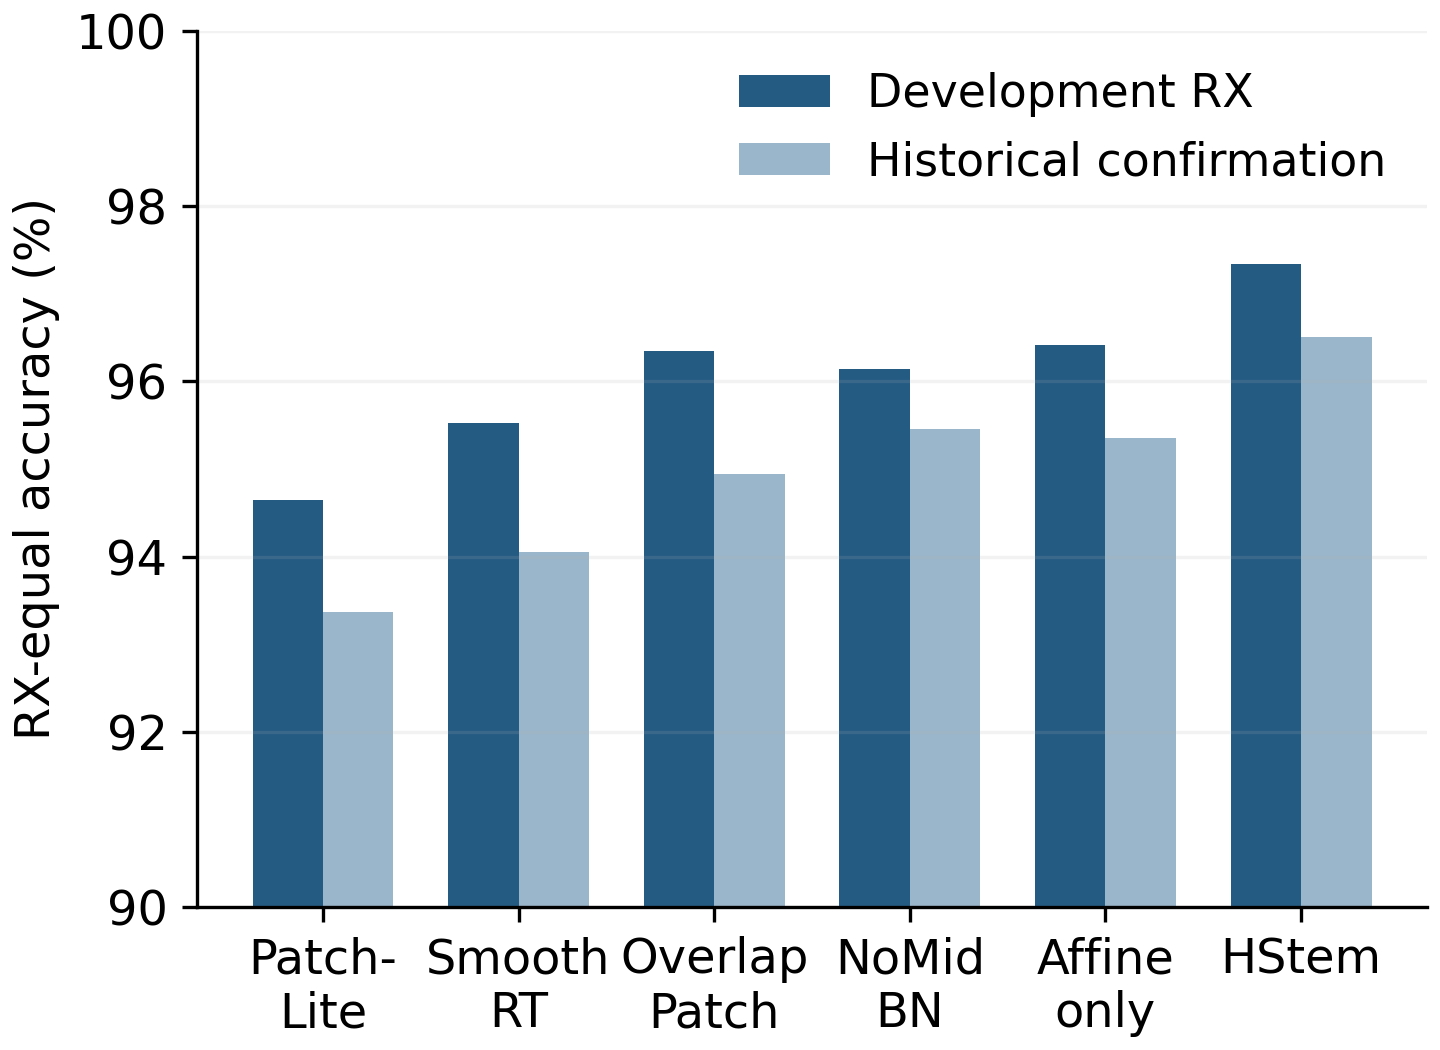
\includegraphics[width=\columnwidth]{mechanism.png}
\caption{Fixed tokenizer variants on development and historical-confirmation receivers. Historical-confirmation values have prior exposure and are descriptive. The paired contrast table, rather than bar ranking alone, determines the mechanism conclusions.}
\label{fig:mechanism}
\end{figure}

\subsection{Affine Restoration Does Not Recover Full BN Performance}
Removing intermediate BN reduces development accuracy from 97.335\% to 96.145\%. Restoring only channel affine parameters raises it to 96.417\%. AffineOnly minus NoMidBN is a small positive 0.272 pp, below the 0.5 pp practical threshold. Full \method{} exceeds AffineOnly by 0.918 pp on average, but only four of six fitted pairs are positive, so that contrast fails the registered stability rule despite its positive interval.

It is therefore inaccurate to attribute the full BN effect merely to the 352 affine parameters. It is also inaccurate to claim that a stable, isolated normalization-statistics mechanism has been established. The worst-RX difference for \method{} versus AffineOnly is -0.717 pp. All four planned contrasts, including these two non-passing practical signals, are reported.

\subsection{Deployment Equivalence Requires Numerical Qualification}
All six trained Smooth-RoundTrip models can be materialized as ordinary convolutions. Across 12,000 source-validation evaluations, the maximum logit difference is zero and every predicted class is unchanged. This verifies a deployment transformation of the trained models; it does not imply that ordinary Patch-Lite training from its original initialization reaches the same weights.

For BN folding, all six hierarchical models fail the pre-fixed $\mathrm{atol}=\mathrm{rtol}=10^{-4}$ logit test under the default TF32-enabled convolution setting. The maximum absolute discrepancy is approximately 0.01957, although all 12,000 predicted classes remain unchanged. A subsequent precision diagnostic disables TF32, preserves checkpoints, inputs, and tolerances, and passes all six models, with maximum discrepancy $5.39\times10^{-5}$. The original failures are retained. This supplementary diagnostic is not represented as the initial preregistered test.

\subsection{Computational and Alignment Boundaries}
\begin{table}[t]
\centering\caption{Recorded same-GPU forward costs. MACs incompletely cover FFT/interpolation/elementwise work. Latency is resident-input p50, without I/O.}
\label{tab:costs}
\setlength{\tabcolsep}{4pt}\footnotesize
\begin{tabular}{lrrr}
\toprule Model & MACs (M) & Batch 1 (ms) & Batch 128 (ms)\\\midrule
Patch-Lite & 55.346 & 2.281 & 13.453\\
Smooth-RoundTrip & 55.346 & 2.373 & 13.514\\
Overlap-Patch & 56.206 & 2.343 & 19.339\\
NoMidBN & 95.028 & 2.429 & 15.645\\
AffineOnly & 95.028 & 2.661 & 16.768\\
HStem & 95.028 & 2.510 & 16.123\\
\bottomrule\end{tabular}
\end{table}

Table~\ref{tab:costs} shows the cost trade-off. \method{} uses fewer parameters than full Patch but approximately 95.028 M counted MACs, versus 55.346 M for Patch-Lite. On the recorded NVIDIA GeForce RTX 4060 Laptop GPU, batch-128 median forward latency is approximately 16.123 ms versus 13.453 ms; single-packet medians are 2.510 and 2.281 ms. MAC counting excludes some FFT, interpolation, and elementwise work. The measurements do not justify a universal speed or energy-efficiency claim.

\begin{table}[t]
\centering\caption{Frozen source-validation digital-shift tests (\%). No receiver-generalization or physical synchronization claim is inferred from these interventions.}
\label{tab:stress}
\setlength{\tabcolsep}{6pt}\footnotesize
\begin{tabular}{lrr}
\toprule Condition & HStem & Patch-Lite\\\midrule
Clean & 98.175 & 95.925\\
Circular $-1$ & 81.167 & 79.417\\
Circular $+1$ & 75.933 & 70.908\\
Circular $-4$ & 21.858 & 22.567\\
Circular $+4$ & 17.775 & 16.983\\
Zero-filled $-4$ & 21.867 & 21.092\\
Zero-filled $+4$ & 17.383 & 17.233\\
Circular $-4$, FFT locked & 21.850 & 22.567\\
Circular $+4$, FFT locked & 17.775 & 16.983\\
\bottomrule\end{tabular}
\end{table}

The frozen source-validation stress tests in Table~\ref{tab:stress} expose a strong alignment limitation. Hierarchical-model accuracy drops from 98.175\% to 21.858\% and 17.775\% under circular shifts of -4 and +4 samples. Patch-Lite also degrades severely. Circular shifts preserve discrete sample content and DFT magnitude up to numerical error. Locking the FFT magnitude view to its clean value changes overall accuracy by at most 0.0083 pp in these tests and does not remove the collapse. Zero-filled shifts cause similar degradation.

These results rule out zero-padding loss or tiny FFT-magnitude differences as sufficient explanations. They do not uniquely identify the responsible phase channel, positional cue, stride, transmitter timing, or receiver circuitry. The corpus supplies fixed windows without adjacent continuous IQ or validated synchronization-error distributions. Circular shifts are consequently digital stress tests, not established models of real acquisition errors. We make no synchronization-robustness claim.

\section{Discussion and Limitations}
\subsection{What the Controls Establish}
The main evidence is a reproducible system comparison within a restricted source budget and aligned representation. The matched patch result reduces a parameter-count explanation. The round-trip control shows that a full-rank change of training coordinates can matter without enlarged support. Expanded support retains an additional observed advantage, but operator and frequency-response differences prevent pure causal attribution. The affine controls similarly constrain, rather than resolve, the normalization explanation.

Materialization and BN folding distinguish properties of training from requirements of deployment. Their verification is finite and numerical. Bitwise equality on the tested source inputs is stronger than matching predicted labels, but is not a mathematical guarantee for arbitrary backends or all possible signals. In particular, default TF32 folding discrepancies must not be erased by reporting only the strict-precision follow-up.

\subsection{What the Evidence Does Not Establish}
The experiments do not isolate a transmitter-only hardware signature from receiver and channel effects. Kernel spectra refer to learned feature coordinates, not measured transmitter RF frequency responses. Cross-receiver performance under this corpus is not proof of hardware invariance. Neither the stronger source-validation stress-test accuracy nor historical-confirmation accuracy is a substitute for new receiver-level evidence.

The cumulative use of development and historical-confirmation receivers limits independent inference. The six receivers withheld from this protocol already have prior-study exposure. A future external evaluation must establish its qualification separately; merely reusing those six receivers would not restore blindness. We do not broaden the paper into a universal LoRa/Wi-Fi method or claim a state-of-the-art ranking against incompatible public protocols.

\subsection{Reproducibility and Relationship Disclosure}
The companion source bundle includes the final protocol, receiver lists, aggregate and per-receiver CSV tables, local-risk records, source provenance hashes, numerical-equivalence checks, and figure-generation scripts. The main manuscript and supplement distinguish inherited components from the tokenizer contribution. Raw data and pre-existing model weights remain subject to their original availability and license terms. The related OOB manuscript is disclosed rather than treated as an independent competing baseline.

\section{Conclusion}
Under the studied aligned, strictly in-band LoRa protocol, a four-stage hierarchical tokenizer improves cross-receiver development accuracy while substantially reducing parameters relative to a full patch projection. Parameter-matched controls and targeted ablations show that RF token formation is consequential, with contributions from parameterization and local-support-related design that are not fully separable. Trained interpolation can be removed from the deployment graph, while BN folding requires explicit precision qualification. Higher arithmetic cost, strong digital-shift sensitivity, and prior receiver exposure define the limits of the present result. The contribution is a bounded tokenizer design and its controlled evidence, not a new theory of RF hardware invariance.

\balance
\bibliographystyle{IEEEtran}
\bibliography{references}
\end{document}
